
%associated with three attributes, i.e., workload $w$, execution rate $\sigma$, and completion time $t$.
%This makes our framework agnostic to the granularity of the resource allocation unit.
%Cores are subject to failures. We assume that core failures are independent and identically distributed (i.i.d.). We do not distinguish between soft and hard failures, assuming that soft failures are handled via software rejuvenation (i.e., rebooting \cite{466961}), while hard failures are handled by replacing the failed components with spares. We adopt the fail-stop fault model, whereby a core stops executing upon failure and failures are detected by other non-failing cores \cite{gartner_faults_1999,cristian_comm_1991}. %When a core fails, the whole execution is suspended until recovery is complete. 

%%%%%%%%%%%%%%%%%%%%%%%%%%%%%%rethinking%%%%%%%%%%%%%%%%%%%%%%
%We assume that core failures are independent and identically distributed (i.i.d.). In the real world, instead, failures are bound to be correlated. Obtaining theoretical results for non-i.i.d. failures is beyond the scope of this work. But note that one cause of correlation is the hierarchical structure of computing platforms (each rack comprises compute nodes, each compute node comprises processors, and each processor comprises cores), which leads to simultaneous failures of a group of cores. Our work applies to such failures since a group of failures can be treated as multiple individual failures that happen at the same time and their recovery can be carried out in parallel.


We use the term core to represent the computing resource allocation unit%(e.g., a
%CPU core, a multi-core CPU, or a cluster node)
~\cite{casanova_inria_2012}. 
We further use $P(\sigma$, $w$, $t)$ to denote a process executing at rate $\sigma$ to complete a workload $w$ by time $t$.
The basic tenet of the Lazy Shadowing resilience model is the concept of shadowing, whereby each process is associated with a {\it lazy} replica. %This guarantees that if one process fails, the other one can still complete the task. 
Assuming a single failure, Lazy Shadowing can be described as follows:
\begin{itemize}
	\item A main process, $P_m(\sigma_m$, $w$, $t_m)$, that executes at the rate of $\sigma_m$ to complete a task of size $w$ at time $t_m$.
	\item A shadow process, $P_s(<\sigma_s^b$ , $\sigma_s^a>$, $w$, $t_s)$, that executes at $\sigma_s^b$ before failure, and $\sigma_s^a$ after failure, to complete a task of size $w$ at time $t_s$.% where $\sigma_s^b$ represents the execution rate before failure, $\sigma_s^a$ the execution rate after failure, $w$ is the task size, and $t_s$ is the completion time.%, which has the same workload $w$. It starts execution simultaneously with the main process at rate $\sigma_b  \le \sigma_m$, but on a different core. Upon failure of the main process, the shadow process will be designated as the new main process, with its rate switched to $\sigma_a$ to catch up. In this case, the completion time is denoted as $t_s$. 
\end{itemize}

The main process and its shadow start executing simultaneously on two different cores. The main process executes at rate $\sigma_m$, while the shadow initially executes at rate $\sigma_s^b \le \sigma_m$. %To avoid simultaneous failure, they are deployed on different cores.
%with the main running at  
%a rate $\sigma_m$ and the lazy shadow at a lower rate $\sigma_s \le \sigma_m$. 
In the absence of failure, the main process completes execution at time 
$t_m = w/\sigma_m$, which immediately triggers the termination of the
shadow. However, if at time $t_f < t_m$ the main process fails, the shadow, which has completed an amount of work $w_b=\sigma_s^b * t_f$, increases its execution rate to $\sigma_s^a$ to complete the task by $t_s$.%, as depicted in Figure~\ref{fig:fail}. More specifically, the shadow completes $\sigma_s * t_f$ work by $t_f$, and finishes the remaining $(w-\sigma_s * t_f)$ work at $\sigma_a$. %The expected completion time, $T$, of the task can be easily computed by integrating $t_s(t_f) * f(t_f)$, where $f(t_f)$ is the probability of a failure occurring at time $t_f$.
The execution dynamics of Lazy Shadowing are depicted in Figure~\ref{fig:sync}.

\begin{figure}[!t]
	\begin{center}
		\subfigure[Main process sucessful completion.]
		{
			\label{fig:succ}
			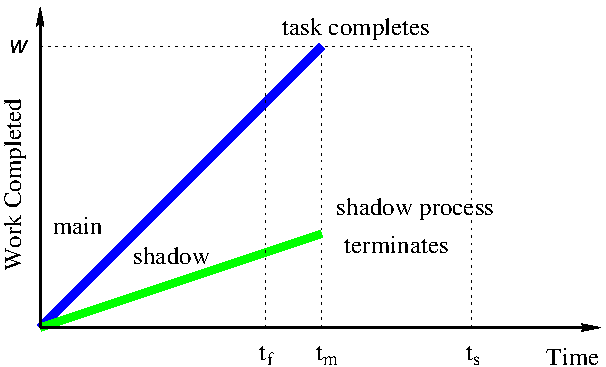
\includegraphics[width=0.40\textwidth]{Figures/succ_new.pdf}
		}
		\subfigure[Main process failure.]
		{
			\label{fig:fail}
			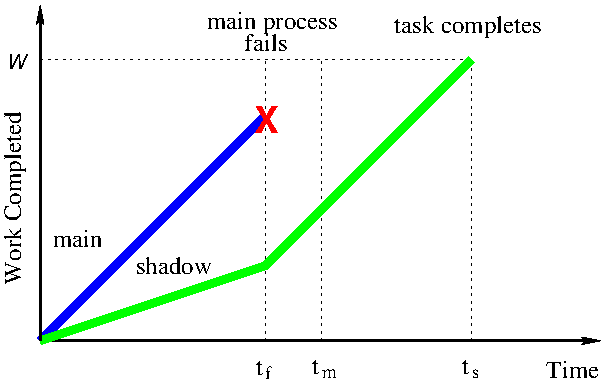
\includegraphics[width=0.40\textwidth]{Figures/fail_new.pdf}
		}
	\end{center}
	\vskip -0.25in 
	\caption{Lazy Shadowing execution dynamics.}
	\label{fig:sync}
\end{figure}

%The execution rate of the shadow before and , 

%For simplicity, we assume the maximum execution rate of a core is 1. In HPC, throughput consideration requires that the rates of the main task, $\sigma_m$, and the shadow after failure, $\sigma_a$, be set to the maximum. 
The execution rates of the shadow, $\sigma_s^b$ and $\sigma_s^a$, can be derived by balancing trade-offs between completion time and energy consumption.
%are determined based on the tolerance of the application to completion time.
For a delay-tolerant, energy-stringent application, $\sigma_s^b$ is set to 0, and the shadow starts executing at the minimum execution rate only upon failure of the main process. %, for maximum energy saving. %, which guarantees additional energy is consumed only upon failure
For a delay-stringent, energy-tolerant application, the shadow starts executing at $\sigma_s^b=\sigma_m$ to guarantee the completion of the task at the specified time $t_m$, regardless of when the failure occurs. 
For delay and energy tolerant applications, a broad spectrum of delay and energy tradeoffs can be explored either empirically or using optimization frameworks.
%For elastic applications, the delay-energy product can be used to derive the execution rate  
%For other applications, $\sigma_s^b$ and $\sigma_s^a$ can be derived by balancing trade-offs between completion time and energy consumption
%however, may still be tuned to manage the trade-offs between completion time and energy consumption. Smaller $\sigma_b$ corresponds to lazier shadowing of the main process.

 %Figure~\ref{fig:succ} illustrates the execution scenario with no failure, while Figure~\ref{fig:fail} depicts the scenario where the main process fails.




%In terms of execution rates, this can be expressed as $\sigma_m=\sigma_a=1$ and $\sigma_s \le 1$.  

%There are multiple ways to control the execution rates of the processes. The most straightforward solution is to allocate a dedicated core for each process while using 
%Dynamic Voltage and Frequency Scaling (DVFS) is a commonly used power management technique 
To control the shadow's execution rate, Dynamic Voltage and Frequency Scaling (DVFS), a commonly used power management technique, can be used. 
The effectiveness of DVFS, however, may be markedly reduced in computational platforms that exhibit saturation of the processor clock frequencies, large static power consumption, or smaller power dynamic range. An alternative to DVFS is to collocate multiple shadows on a single core, runing at maximum rate. Time sharing can then be used to achieve the desired execution rates of the shadows. Given our focus on exetreme-scale, multi-core computing infrastructure, we will use collocation for execution rate control.  
%Recent development in processor and memory technology which results in the saturation of the processor clock frequencies, larger static power consumption, and smaller power dynamic range can markedly reduce the effectiveness of DVFS

 %to tune the frequency of the core. An alternative is to collocate multiple processes on a core, which runs at the maximum rate, and execute the processes in a time sharing manner. In the rest of this paper, we will focus on the idea of collocation in the discussion of applying Lazy Shadowing to HPC applications.  



